\section{Additional Experimental Results}
\label{app:results}

\new{\subsection{Surveyed Audio-Native Models}\label{app:audio-native-audit}}

\new{\tauvoice{} evaluates three audio-native models in the main body (\S\ref{sec:experiments}); this appendix documents the broader survey behind that selection. As of March 2026, we surveyed the audio-native models listed in Table~\ref{tab:audio-native-audit}. The two inclusion criteria are realtime full-duplex audio \emph{and} native tool calling, both required because \tauvoice{} is a grounded, tool-use benchmark; the disqualified models satisfy the first criterion but not the second, since their published documentation does not describe tool-calling support from their audio-conditioned head. Amazon Nova 2 Sonic qualifies on both axes but was deprioritized as another closed-source provider unlikely to add qualitatively different insight to the three already evaluated.}\why{addresses macs W4 + follow-up; vw95 W3}

\begin{table}[h]
\caption{\new{Audio-native models surveyed for \tauvoice{} evaluation, as of March 2026. Realtime full-duplex audio = streaming bidirectional audio with voice-activity-detected turn-taking. Native tool calling = the model supports tool calls directly from its audio-conditioned head, without an external ASR$\to$LLM cascade. Both criteria are required for inclusion (\S\ref{sec:experiments}).}\why{addresses macs W4}}
\label{tab:audio-native-audit}
\centering
\begin{small}
\resizebox{\columnwidth}{!}{%
\new{\begin{tabular}{@{}lccc@{}}
\toprule
\textbf{Model} & \makecell{\textbf{Realtime}\\\textbf{full-duplex audio}} & \makecell{\textbf{Native}\\\textbf{tool calling}} & \makecell{\textbf{Evaluated}\\\textbf{in \tauvoice{}}} \\
\midrule
\multicolumn{4}{l}{\textit{Qualifying (both criteria satisfied)}} \\
OpenAI Realtime~\cite{openai_introducing_2025} & \checkmark & \checkmark & \checkmark \\
Gemini Live~\cite{vertex_ai_gemini_2025} & \checkmark & \checkmark & \checkmark \\
xAI Voice Agent~\cite{xai_grok_voice_2025} & \checkmark & \checkmark & \checkmark \\
Amazon Nova 2 Sonic~\cite{amazon_nova_sonic_2025} & \checkmark & \checkmark & \xmark$^{\dagger}$ \\
\midrule
\multicolumn{4}{l}{\textit{Realtime full-duplex audio, but no native tool calling}} \\
NTPP~\cite{wang_ntpp_2025} & \checkmark & \xmark & \xmark \\
LLaMA-Omni~\cite{fang_llama-omni_2025} & \checkmark & \xmark & \xmark \\
SALMONN-omni~\cite{yu_salmonn-omni_2025} & \checkmark & \xmark & \xmark \\
Moshi~\cite{defossez_moshi_2024} & \checkmark & \xmark & \xmark \\
PersonaPlex~\cite{nvidia_personaplex_2026} & \checkmark & \xmark & \xmark \\
MiniCPM-o 4.5~\cite{openbmb_minicpm-o_2026} & \checkmark & \xmark & \xmark \\
Qwen-Omni-Realtime~\cite{qwen_omni_realtime_2025} & \checkmark & \xmark & \xmark \\
\bottomrule
\end{tabular}}%
}
\end{small}
\\[0.5em]
\new{\footnotesize $^{\dagger}$ Qualifies on both axes but deprioritized as another closed-source provider unlikely to add qualitatively different insight beyond the three already evaluated.}\why{addresses macs follow-up}
\end{table}

\subsection{Voice Interaction Quality: Full Metric Breakdown}
\label{app:voice-metrics-detail}

Table~\ref{tab:voice-quality-detail} provides the full breakdown of voice interaction metrics. Columns are grouped by: \textbf{Latency} ($L_R$ = Response Latency, $L_Y$ = Yield Latency), \textbf{Responsiveness} ($R_R$ = Response Rate, $R_Y$ = Yield Rate), \textbf{Interrupt} ($I_A$ = Agent Interruption Rate), and \textbf{Selectivity} ($S_{BC}$ = Backchannel Correct, $S_{VT}$ = Vocal Tic Correct, $S_{ND}$ = Non-Directed Correct). For $L_R$, $R_R$, and $I_A$, separate columns show Clean (C) and Realistic (R) speech conditions; other metrics are evaluated on Realistic only.

\begin{table*}[h]
\caption{Voice interaction quality metrics---full breakdown (Realistic condition). \textbf{Bold} indicates best per domain. $\uparrow$ = higher is better, $\downarrow$ = lower is better.}
\label{tab:voice-quality-detail}
\centering
\begin{small}
\resizebox{\textwidth}{!}{%
\begin{tabular}{@{}ll|cc|c|cc|c|cc|ccc@{}}
\toprule
 & & \multicolumn{3}{c|}{\textbf{Latency}$\downarrow$} & \multicolumn{3}{c|}{\textbf{Responsiveness}$\uparrow$} & \multicolumn{2}{c|}{\textbf{Interrupt}$\downarrow$} & \multicolumn{3}{c}{\textbf{Selectivity}$\uparrow$} \\
 & & \multicolumn{2}{c|}{$L_R$} & \multirow{2}{*}{$L_Y$} & \multicolumn{2}{c|}{$R_R$} & \multirow{2}{*}{$R_Y$} & \multicolumn{2}{c|}{$I_A$} & \multirow{2}{*}{$S_{BC}$} & \multirow{2}{*}{$S_{VT}$} & \multirow{2}{*}{$S_{ND}$} \\
\textbf{Domain} & {\textbf{Model}} & C & R & & C & R & & C & R & & & \\
\midrule
\multirow{3}{*}{All} & {\texttt{gemini-live-2.5}} & 1.40s & 1.43s & 0.86s & 96\% & 81\% & 56\% & 7\% & 21\% & 85\% & 34\% & \textbf{45\%} \\
 & {\texttt{gpt-realtime-1.5}} & 1.69s & 1.39s & \textbf{0.42s} & \textbf{99\%} & \textbf{100\%} & \textbf{100\%} & \textbf{1\%} & \textbf{14\%} & 2\% & 5\% & 10\% \\
 & {\texttt{grok-voice}} & \textbf{1.05s} & \textbf{1.15s} & 1.15s & 92\% & 91\% & 75\% & 44\% & 84\% & \textbf{93\%} & \textbf{58\%} & 21\% \\
\midrule
\multirow{3}{*}{Retail} & {\texttt{gemini-live-2.5}} & 1.50s & 1.45s & 0.86s & 96\% & 79\% & 61\% & 6\% & 17\% & 91\% & 28\% & \textbf{45\%} \\
 & {\texttt{gpt-realtime-1.5}} & 1.81s & 1.39s & \textbf{0.43s} & \textbf{99\%} & \textbf{100\%} & \textbf{100\%} & \textbf{1\%} & \textbf{15\%} & 3\% & 6\% & 8\% \\
 & {\texttt{grok-voice}} & \textbf{1.09s} & \textbf{1.12s} & 1.18s & 84\% & 91\% & 70\% & 29\% & 77\% & \textbf{93\%} & \textbf{61\%} & 22\% \\
\midrule
\multirow{3}{*}{Airline} & {\texttt{gemini-live-2.5}} & 1.40s & 1.46s & 0.73s & 95\% & 80\% & 57\% & 6\% & 19\% & 89\% & 40\% & \textbf{55\%} \\
 & {\texttt{gpt-realtime-1.5}} & 1.79s & 1.43s & \textbf{0.42s} & \textbf{99\%} & \textbf{100\%} & \textbf{100\%} & \textbf{1\%} & \textbf{14\%} & 2\% & 6\% & 7\% \\
 & {\texttt{grok-voice}} & \textbf{1.08s} & \textbf{1.18s} & 1.12s & 93\% & 91\% & 77\% & 62\% & 83\% & \textbf{91\%} & \textbf{59\%} & 20\% \\
\midrule
\multirow{3}{*}{Telecom} & {\texttt{gemini-live-2.5}} & 1.28s & 1.38s & 0.99s & 96\% & 82\% & 50\% & 8\% & 26\% & 75\% & 33\% & \textbf{34\%} \\
 & {\texttt{gpt-realtime-1.5}} & 1.48s & 1.35s & \textbf{0.41s} & \textbf{100\%} & \textbf{100\%} & \textbf{100\%} & \textbf{1\%} & \textbf{12\%} & 0\% & 3\% & 13\% \\
 & {\texttt{grok-voice}} & \textbf{0.98s} & \textbf{1.16s} & 1.16s & 99\% & 93\% & 78\% & 39\% & 93\% & \textbf{94\%} & \textbf{55\%} & 22\% \\
\bottomrule
\end{tabular}
}
\end{small}
\end{table*}

% TODO: Add per-task breakdown, statistical significance tests


\subsection{Qualitative Error Analysis}
\label{app:qualitative-analysis}

We conducted a qualitative analysis of task failures to understand error sources and types. We annotated all failed simulations from two analysis cohorts: (1) Voice-Fragile (43 simulations across 20 tasks passing in text but failing in Clean audio), and (2) Noise-Fragile (48 simulations across 19 tasks passing in Clean but failing in Realistic audio).

\paragraph{Qualitative Annotations.}
Table~\ref{tab:full-notes-both} shows the qualitative annotations for each failed simulation.

\begin{table*}[h]
\caption{Qualitative error annotations for task completion failures. Left: Voice-Fragile cohort (43 simulations from Clean audio setting). Right: Noise-Fragile cohort (48 simulations from Realistic audio setting).}
\label{tab:full-notes-both}
\centering
\begin{small}
\begin{minipage}{0.48\textwidth}
\centering
\textbf{Voice-Fragile}\\[0.5em]
\input{results/full_notes_text_vs_clean_audio}
\end{minipage}
\hfill
\begin{minipage}{0.48\textwidth}
\centering
\textbf{Noise-Fragile}\\[0.5em]
\input{results/full_notes_clean_vs_realistic_audio}
\end{minipage}
\end{small}
\end{table*}

\paragraph{Error Type Definitions.}
We categorize errors into six types based on observed failure patterns:

\begin{itemize}[nosep,leftmargin=*]
    \item \textbf{Logical} (Agent or User): Reasoning or execution errors, including incorrect tool call arguments/formatting, taking wrong actions (cancelling/modifying wrong items), failing to follow instructions (not asking for spelling, not confirming), or losing track of conversation state.
    
    \item \textbf{Transcription} (Agent): Speech-to-text errors where the agent incorrectly transcribes user speech, most commonly during authentication when users spell names/emails letter-by-letter, or when transcribing specific user requests.
    
    \item \textbf{Hallucination} (Agent or User): Agent fabricates information (e.g., inventing item IDs, hallucinating order details) or user simulator states information not present in the task instructions.
    
    \item \textbf{VAD/Unresponsive} (Agent): Voice Activity Detection errors where the agent fails to detect user speech, or agent goes silent for an extended period despite multiple user check-ins.
    
    \item \textbf{Timeout} (Agent): Agent could not resolve the call within the 20-minute simulation limit, typically due to being too slow or verbose.
    
    \item \textbf{Early Termination} (User): User ends the call prematurely before the task is fully completed, often due to ambiguous communication where user assumes the task is done when it is not.
\end{itemize}

\new{\subsection{Skill-Axis Classification of Agent-Attributable Failures}\label{app:skill-classification}}

\new{To assess what type of capability the benchmark's task-completion failures are surfacing, we re-cut the 77 agent-attributable failures (34 Voice-Fragile + 43 Noise-Fragile, matching the 79\%/90\% agent shares in Table~\ref{tab:combined-error-analysis}) along a third axis: \emph{the skill whose absence was the proximal cause of failure}. This axis is orthogonal to the error-type taxonomy above---e.g., a transcription error and a logical error can both reflect the same underlying spelling deficit---and is intended to answer whether failures are concentrated in domain-specific policy knowledge or in general conversational competence.}\why{addresses vw95 W2: data backing for the commonsense vs. policy framing}

\new{\paragraph{Methodology.} The 77 rows correspond to the agent-attributable subset of the reconciled annotations from \S\ref{sec:analysis} (after the 84\%-agreement inter-rater pass and resolution discussion). A single annotator reviewed each row's error type, the free-text notes, and the arbitration notes where present, assigning it to exactly one of six mutually exclusive skill buckets. The assignment rule is ``what skill, if present, would have prevented this failure?''---the proximal absent skill, not the union of contributing factors. Per-row rationales accompany the released annotations.}\why{addresses vw95 W2}

\new{\paragraph{Skill buckets.} Five buckets capture domain-agnostic commonsense conversational skills; one captures domain-specific policy knowledge:}\why{addresses vw95 W2}

\new{\begin{itemize}[nosep,leftmargin=*]
    \item \textbf{Spelling}: Agent transcribes a spelled-out name, email, or ID incorrectly, blocking authentication or producing a downstream lookup miss.
    \item \textbf{Conversational grounding}: Agent executes an irreversible action without explicit user confirmation, or fails to share information the user needs to make the next decision.
    \item \textbf{Conversational honesty}: Agent claims an action was performed when no corresponding tool call exists in the trace, or acts on a wrong item/entity.
    \item \textbf{Multi-part request tracking}: User makes a compound request; agent completes one part and treats the call as resolved.
    \item \textbf{Arithmetic / self-consistency}: Agent makes an arithmetic error (refund total, line-item sum) or contradicts an earlier statement in the same call.
    \item \textbf{Policy-specific knowledge}: Failure requires knowledge of a domain-specific rule in the agent's policy prompt (e.g., one-time-process rule, refund-method policy).
\end{itemize}}\why{addresses vw95 W2}

\new{\paragraph{Results.} Table~\ref{tab:skill-classification} shows the distribution. 73/77 (94.8\%) of agent-attributable failures fall into the five commonsense buckets; only 4/77 (5.2\%) require domain-specific policy knowledge. Spelling (35.1\%) and conversational grounding (31.2\%) dominate, accounting for nearly two-thirds of all agent-attributable failures.}\why{addresses vw95 W2}

\begin{table}[h]
\caption{\new{Skill-axis classification of the 77 agent-attributable failures. Five buckets are domain-agnostic commonsense conversational skills; one is domain-specific policy knowledge.}\why{addresses vw95 W2}}
\label{tab:skill-classification}
\centering
\begin{small}
\new{\begin{tabular}{@{}lrr@{}}
\toprule
\textbf{Skill bucket} & \textbf{Count} & \textbf{\%} \\
\midrule
\multicolumn{3}{l}{\textit{Domain-agnostic commonsense}} \\
Spelling & 27 & 35.1\% \\
Conversational grounding & 24 & 31.2\% \\
Conversational honesty & 13 & 16.9\% \\
Multi-part request tracking & 5 & 6.5\% \\
Arithmetic / self-consistency & 4 & 5.2\% \\
\midrule
\textbf{Commonsense subtotal} & \textbf{73} & \textbf{94.8\%} \\
\midrule
\multicolumn{3}{l}{\textit{Domain-specific}} \\
Policy-specific knowledge & 4 & 5.2\% \\
\midrule
\textbf{Total} & \textbf{77} & \textbf{100\%} \\
\bottomrule
\end{tabular}}
\end{small}
\end{table}

\new{\paragraph{Discussion.} The concentration in commonsense buckets indicates that the voice-text gap reported in \S\ref{sec:results} is not primarily a question of domain knowledge---the agents already have the relevant policy text in their prompts---but of general conversational competence under voice conditions. Spelling failures in particular compound under realistic audio (Table~\ref{tab:ablation-single}), since accents and background noise degrade exactly the part of the interaction (letter-by-letter authentication) the agent depends on to begin acting.}\why{addresses vw95 W2}

\new{\subsection{Simulator Realism Validation}\label{app:simulator-realism}}

\new{To validate that the voice user simulator produces interactions that resemble realistic caller behavior, we conducted a small human annotation study.}\why{addresses macs Q3/Q4}

\new{\paragraph{Methodology.} Two annotators independently rated 60 simulations stratified across domains and speech-complexity conditions on a 1--4 Likert scale (1 = clearly unrealistic, 4 = indistinguishable from a real caller). Each simulation was rated along six dimensions:}\why{addresses macs Q3/Q4}

\new{\begin{itemize}[nosep,leftmargin=*]
    \item \textbf{Voice prosody}: pitch, rhythm, and intonation of the synthesized caller speech.
    \item \textbf{Audio environment realism}: plausibility of the simulated background audio (noise, ambient sounds, intermittent events).
    \item \textbf{Turn-taking naturalness}: timing and flow of speaker transitions.
    \item \textbf{Backchannel naturalness}: realism of acknowledgement tokens (``mm-hmm'', ``okay'').
    \item \textbf{Interruption behavior}: appropriateness and frequency of mid-utterance interjections.
    \item \textbf{Behavioral plausibility}: holistic judgment of whether the caller behaves like a real human across the whole call.
\end{itemize}}\why{addresses macs Q3/Q4}

\new{\paragraph{Results.} Table~\ref{tab:simulator-realism} reports the per-dimension means averaged across the two annotators. Averaging across the six dimensions, the simulator achieves an overall mean of 3.1/4, with 83\% of all individual ratings at 3 or above. Within-1 inter-rater agreement --- the fraction of (simulation, dimension) pairs on which the two raters' scores are within one point of each other --- is 94\%, suggesting consistent perception of simulator quality across annotators. Figure~\ref{fig:simulator-realism-distribution} shows the underlying per-rater distributions: five dimensions display overlapping right-skewed shapes, while on \emph{audio environment realism} Rater B did not differentiate (all 60 ratings = 3), so the table's 3.3 entry for that dimension reflects Rater A's variation only.}\why{addresses macs Q3/Q4; coauthor: surface per-rater distributions}

\begin{table}[h]
\caption{\new{Simulator realism ratings, averaged across two annotators on 60 simulations (1--4 scale; higher is better). Overall row is the mean across the six dimensions.}\why{addresses macs Q3/Q4}}
\label{tab:simulator-realism}
\centering
\begin{small}
\new{\begin{tabular}{@{}lc@{}}
\toprule
\textbf{Dimension} & \textbf{Mean rating} \\
\midrule
Voice prosody & 2.6 / 4 \\
Audio environment realism & 3.3 / 4 \\
Turn-taking naturalness & 3.1 / 4 \\
Backchannel naturalness & \textbf{3.5 / 4} \\
Interruption behavior & 3.0 / 4 \\
Behavioral plausibility (holistic) & 3.1 / 4 \\
\midrule
\textbf{Overall (mean across dimensions)} & \textbf{3.1 / 4} \\
\bottomrule
\end{tabular}}
\end{small}
\end{table}

\begin{figure*}[h]
\centering
\new{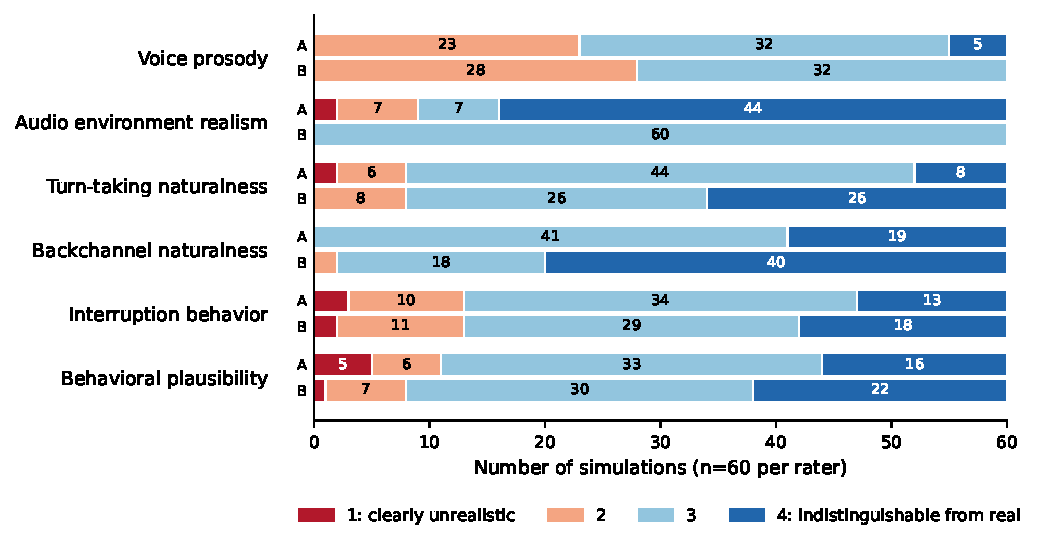
\includegraphics[width=0.85\textwidth]{results/simulator_realism_distribution.pdf}}
\caption{\new{Per-rater rating distributions for the simulator-realism study (\S\ref{app:simulator-realism}; $n=60$ simulations per rater). Stacked bars show how each rater (A, B) distributed their 1--4 Likert ratings across the six dimensions.}\why{addresses coauthor: surface per-rater distributions}}
\label{fig:simulator-realism-distribution}
\end{figure*}

\new{\paragraph{Discussion.} The dimensions most directly relevant to task evaluation---turn-taking, interruption behavior, backchanneling, and overall behavioral plausibility---all score at or above 3.0/4, supporting the use of the simulator as a controllable substitute for human callers in this benchmark. The weakest dimension is voice prosody (2.6/4), consistent with our deliberate choice (\S\ref{sec:conclusion}) not to evaluate agent speech generation quality and to treat TTS-synthesized caller audio as indicative rather than definitive. This study is not a substitute for evaluation with real human callers, which we list as future work (\S\ref{sec:conclusion}); rather, it provides a check that the dimensions of simulator behavior that most directly affect agent task completion are acceptably realistic.}\why{addresses macs Q3/Q4}

\subsection{Statistical Reliability Analysis}
\label{app:stat-sig}

\new{To assess statistical reliability, we conducted 2 independent runs per condition across all three domains (Airline $n=50$, Retail $n=114$, Telecom $n=114$). We use paired permutation tests rather than trial-level confidence intervals: for each pair of conditions, we compute per-task mean success rates, pair observations by task ID, and test whether the paired differences are systematically non-zero (100k permutations, two-sided). $p$-values are Holm-Bonferroni corrected within each (domain, model) group to control for multiple comparisons; for the combined view, correction is applied within each model across all comparisons. Because rates are pooled across both runs, they may differ slightly from the single-run rates reported in the main results.}\why{addresses beyN W4/Q5}\old{To assess statistical reliability, we conducted 2 independent runs per condition on the Retail domain (n=114 tasks per run, 228 simulations per condition). We use paired permutation tests rather than trial-level confidence intervals: for each pair of conditions, we compute per-task mean success rates, pair observations by task ID (114 paired observations), and test whether the paired differences are systematically non-zero (100k permutations, two-sided). P-values are Holm-Bonferroni corrected within each provider group to control for multiple comparisons. Because rates are pooled across both runs, they may differ slightly from the single-run rates reported in the main results.}

\new{Two patterns hold across all three domains (Tables~\ref{tab:stat-sig} and~\ref{tab:stat-sig-per-domain}). First, the gap between voice and reasoning-text (GPT-5) is large and significant in every domain and for every model (all $p < 0.001$). Second, the Clean-to-Realistic degradation holds in Retail for all models, but in Airline and Telecom it is only significant for \texttt{grok-voice}. The most notable per-domain deviation is in Telecom, where \texttt{grok-voice}'s Clean rate (57.5\%) significantly \emph{exceeds} the non-reasoning text baseline ($+$20.6pp, $p < 0.001$); this pulls the combined non-reasoning Text$\,\to\,$Clean gap for \texttt{grok-voice} to non-significance ($p = 0.231$), but the anomaly disappears under Realistic conditions where Text$\,\to\,$Realistic is significant for all three models.}\why{addresses beyN W4/Q5}\old{Table~\ref{tab:stat-sig} confirms that both key gaps are statistically significant: (1) the text-to-Clean gap---all providers show significant drops from both text baselines ($p < 0.05$), including the narrowest gap between GPT-4.1 (76.3\%) and OpenAI Clean (67.5\%, $\Delta = -8.8$pp, $p = 0.032$); and (2) the Clean-to-Realistic gap---all three providers show significant degradation (Google $\Delta = -13.2$pp, $p = 0.026$; OpenAI $\Delta = -24.6$pp, $p < 0.001$; xAI $\Delta = -13.2$pp, $p = 0.044$).}

\old{Under Clean conditions, OpenAI (67.5\%) is clearly separated from xAI (50.0\%) and Google (42.1\%). Under Realistic conditions, OpenAI remains strongest (43.0\%), followed by xAI (36.8\%) and Google (28.9\%). The full set of pairwise comparisons across all five speech complexity conditions (Clean, Audio-only, Accents-only, Behavior-only, and Realistic) is available in the supplementary materials.}

\begin{table}[h]
\caption{\new{Pairwise statistical significance pooled across all three domains (Airline, Retail, Telecom; 2 runs each). Text (NR) = GPT-4.1; Text (R) = GPT-5. All $p$-values are Holm-Bonferroni corrected paired permutation tests (100k permutations, paired by task ID).}\why{addresses beyN W4/Q5}\old{Pairwise statistical significance for Retail domain (2 runs, n=114 tasks each). Text (NR) = GPT-4.1; Text (R) = GPT-5. All $p$-values are Holm-Bonferroni corrected paired permutation tests.}}
\label{tab:stat-sig}
\centering
\begin{small}
\begin{tabular}{llrrrc}
\toprule
\textbf{Comparison} & {\textbf{Model}} & \textbf{Rate A} & \textbf{Rate B} & \textbf{$\Delta$ (pp)} & \textbf{$p$ (adj)} \\
\midrule
\multirow{3}{*}{Text (NR) $\to$ Clean} & {\texttt{gemini-live-2.5}} & 55.9\% & 30.6\% & $-$25.3 & $<$0.001 \\
 & {\texttt{gpt-realtime-1.5}} & 55.9\% & 47.8\% & $-$8.0 & 0.001 \\
 & {\texttt{grok-voice}} & 55.9\% & 52.0\% & $-$3.9 & 0.231 \\
\midrule
\multirow{3}{*}{Text (NR) $\to$ Realistic} & {\texttt{gemini-live-2.5}} & 55.9\% & 24.3\% & $-$31.6 & $<$0.001 \\
 & {\texttt{gpt-realtime-1.5}} & 55.9\% & 33.6\% & $-$22.2 & $<$0.001 \\
 & {\texttt{grok-voice}} & 55.9\% & 36.0\% & $-$19.9 & $<$0.001 \\
\midrule
\multirow{3}{*}{Text (R) $\to$ Clean} & {\texttt{gemini-live-2.5}} & 85.2\% & 30.6\% & $-$54.6 & $<$0.001 \\
 & {\texttt{gpt-realtime-1.5}} & 85.2\% & 47.8\% & $-$37.3 & $<$0.001 \\
 & {\texttt{grok-voice}} & 85.2\% & 52.0\% & $-$33.2 & $<$0.001 \\
\midrule
\multirow{3}{*}{Text (R) $\to$ Realistic} & {\texttt{gemini-live-2.5}} & 85.2\% & 24.3\% & $-$60.9 & $<$0.001 \\
 & {\texttt{gpt-realtime-1.5}} & 85.2\% & 33.6\% & $-$51.5 & $<$0.001 \\
 & {\texttt{grok-voice}} & 85.2\% & 36.0\% & $-$49.2 & $<$0.001 \\
\midrule
\multirow{3}{*}{Clean $\to$ Realistic} & {\texttt{gemini-live-2.5}} & 30.6\% & 24.3\% & $-$6.3 & 0.002 \\
 & {\texttt{gpt-realtime-1.5}} & 47.8\% & 33.6\% & $-$14.2 & $<$0.001 \\
 & {\texttt{grok-voice}} & 52.0\% & 36.0\% & $-$16.0 & $<$0.001 \\
\bottomrule
\end{tabular}

\end{small}
\end{table}

\begin{table}[h]
\caption{\new{Per-domain pairwise statistical significance (2 runs per condition). Text (NR) = GPT-4.1; Text (R) = GPT-5. All $p$-values are Holm-Bonferroni corrected paired permutation tests (100k permutations, paired by task ID, corrected within each (domain, model) group).}\why{addresses beyN W4/Q5}}
\label{tab:stat-sig-per-domain}
\centering
\begin{small}
\begin{tabular}{lllrrrc}
\toprule
{\textbf{Domain}} & \textbf{Comparison} & {\textbf{Model}} & \textbf{Rate A} & \textbf{Rate B} & \textbf{$\Delta$ (pp)} & \textbf{$p$ (adj)} \\
\midrule
\multirow{15}{*}{Airline ($n=50$)}
 & \multirow{3}{*}{Text (NR) $\to$ Clean} & {\texttt{gemini-live-2.5}} & 52.5\% & 29.0\% & $-$23.5 & $<$0.001 \\
 &  & {\texttt{gpt-realtime-1.5}} & 52.5\% & 51.0\% & $-$1.5 & 0.851 \\
 &  & {\texttt{grok-voice}} & 52.5\% & 44.0\% & $-$8.5 & 0.217 \\
\cmidrule(l){2-7}
 & \multirow{3}{*}{Text (NR) $\to$ Realistic} & {\texttt{gemini-live-2.5}} & 52.5\% & 30.0\% & $-$22.5 & 0.002 \\
 &  & {\texttt{gpt-realtime-1.5}} & 52.5\% & 41.0\% & $-$11.5 & 0.066 \\
 &  & {\texttt{grok-voice}} & 52.5\% & 30.0\% & $-$22.5 & 0.009 \\
\cmidrule(l){2-7}
 & \multirow{3}{*}{Text (R) $\to$ Clean} & {\texttt{gemini-live-2.5}} & 83.0\% & 29.0\% & $-$54.0 & $<$0.001 \\
 &  & {\texttt{gpt-realtime-1.5}} & 83.0\% & 51.0\% & $-$32.0 & $<$0.001 \\
 &  & {\texttt{grok-voice}} & 83.0\% & 44.0\% & $-$39.0 & $<$0.001 \\
\cmidrule(l){2-7}
 & \multirow{3}{*}{Text (R) $\to$ Realistic} & {\texttt{gemini-live-2.5}} & 83.0\% & 30.0\% & $-$53.0 & $<$0.001 \\
 &  & {\texttt{gpt-realtime-1.5}} & 83.0\% & 41.0\% & $-$42.0 & $<$0.001 \\
 &  & {\texttt{grok-voice}} & 83.0\% & 30.0\% & $-$53.0 & $<$0.001 \\
\cmidrule(l){2-7}
 & \multirow{3}{*}{Clean $\to$ Realistic} & {\texttt{gemini-live-2.5}} & 29.0\% & 30.0\% & $+$1.0 & 1.000 \\
 &  & {\texttt{gpt-realtime-1.5}} & 51.0\% & 41.0\% & $-$10.0 & 0.112 \\
 &  & {\texttt{grok-voice}} & 44.0\% & 30.0\% & $-$14.0 & 0.015 \\
\midrule
\multirow{15}{*}{Retail ($n=114$)}
 & \multirow{3}{*}{Text (NR) $\to$ Clean} & {\texttt{gemini-live-2.5}} & 76.3\% & 42.1\% & $-$34.2 & $<$0.001 \\
 &  & {\texttt{gpt-realtime-1.5}} & 76.3\% & 67.5\% & $-$8.8 & 0.032 \\
 &  & {\texttt{grok-voice}} & 76.3\% & 50.0\% & $-$26.3 & $<$0.001 \\
\cmidrule(l){2-7}
 & \multirow{3}{*}{Text (NR) $\to$ Realistic} & {\texttt{gemini-live-2.5}} & 76.3\% & 28.9\% & $-$47.4 & $<$0.001 \\
 &  & {\texttt{gpt-realtime-1.5}} & 76.3\% & 43.0\% & $-$33.3 & $<$0.001 \\
 &  & {\texttt{grok-voice}} & 76.3\% & 36.8\% & $-$39.5 & $<$0.001 \\
\cmidrule(l){2-7}
 & \multirow{3}{*}{Text (R) $\to$ Clean} & {\texttt{gemini-live-2.5}} & 81.6\% & 42.1\% & $-$39.5 & $<$0.001 \\
 &  & {\texttt{gpt-realtime-1.5}} & 81.6\% & 67.5\% & $-$14.0 & $<$0.001 \\
 &  & {\texttt{grok-voice}} & 81.6\% & 50.0\% & $-$31.6 & $<$0.001 \\
\cmidrule(l){2-7}
 & \multirow{3}{*}{Text (R) $\to$ Realistic} & {\texttt{gemini-live-2.5}} & 81.6\% & 28.9\% & $-$52.6 & $<$0.001 \\
 &  & {\texttt{gpt-realtime-1.5}} & 81.6\% & 43.0\% & $-$38.6 & $<$0.001 \\
 &  & {\texttt{grok-voice}} & 81.6\% & 36.8\% & $-$44.7 & $<$0.001 \\
\cmidrule(l){2-7}
 & \multirow{3}{*}{Clean $\to$ Realistic} & {\texttt{gemini-live-2.5}} & 42.1\% & 28.9\% & $-$13.2 & 0.026 \\
 &  & {\texttt{gpt-realtime-1.5}} & 67.5\% & 43.0\% & $-$24.6 & $<$0.001 \\
 &  & {\texttt{grok-voice}} & 50.0\% & 36.8\% & $-$13.2 & 0.044 \\
\midrule
\multirow{15}{*}{Telecom ($n=114$)}
 & \multirow{3}{*}{Text (NR) $\to$ Clean} & {\texttt{gemini-live-2.5}} & 36.8\% & 19.7\% & $-$17.1 & $<$0.001 \\
 &  & {\texttt{gpt-realtime-1.5}} & 36.8\% & 26.8\% & $-$10.1 & 0.014 \\
 &  & {\texttt{grok-voice}} & 36.8\% & 57.5\% & $+$20.6 & $<$0.001 \\
\cmidrule(l){2-7}
 & \multirow{3}{*}{Text (NR) $\to$ Realistic} & {\texttt{gemini-live-2.5}} & 36.8\% & 17.1\% & $-$19.7 & $<$0.001 \\
 &  & {\texttt{gpt-realtime-1.5}} & 36.8\% & 21.1\% & $-$15.8 & 0.002 \\
 &  & {\texttt{grok-voice}} & 36.8\% & 37.7\% & $+$0.9 & 0.916 \\
\cmidrule(l){2-7}
 & \multirow{3}{*}{Text (R) $\to$ Clean} & {\texttt{gemini-live-2.5}} & 89.7\% & 19.7\% & $-$70.0 & $<$0.001 \\
 &  & {\texttt{gpt-realtime-1.5}} & 89.7\% & 26.8\% & $-$62.9 & $<$0.001 \\
 &  & {\texttt{grok-voice}} & 89.7\% & 57.5\% & $-$32.2 & $<$0.001 \\
\cmidrule(l){2-7}
 & \multirow{3}{*}{Text (R) $\to$ Realistic} & {\texttt{gemini-live-2.5}} & 89.7\% & 17.1\% & $-$72.6 & $<$0.001 \\
 &  & {\texttt{gpt-realtime-1.5}} & 89.7\% & 21.1\% & $-$68.6 & $<$0.001 \\
 &  & {\texttt{grok-voice}} & 89.7\% & 37.7\% & $-$52.0 & $<$0.001 \\
\cmidrule(l){2-7}
 & \multirow{3}{*}{Clean $\to$ Realistic} & {\texttt{gemini-live-2.5}} & 19.7\% & 17.1\% & $-$2.6 & 0.062 \\
 &  & {\texttt{gpt-realtime-1.5}} & 26.8\% & 21.1\% & $-$5.7 & 0.059 \\
 &  & {\texttt{grok-voice}} & 57.5\% & 37.7\% & $-$19.7 & $<$0.001 \\
\bottomrule
\end{tabular}

\end{small}
\end{table}

\new{\subsection{ASR-Enabled Evaluation}\label{app:asr-enabled}}

\new{We ran a preliminary single-run evaluation on Retail ($n=114$) in which the user simulator perceives the agent through Deepgram Nova-3 streaming ASR (telephony $\mu$-law @ 8\,kHz, finalized segments) rather than the agent's native transcript. Both the text-to-voice gap and the Clean-to-Realistic degradation persist with comparable magnitude (Table~\ref{tab:asr-enabled}); formal significance testing is deferred to future work.}\why{addresses beyN follow-up and vw95 follow-up}

\begin{table}[h]
\caption{\new{ASR-enabled vs.\ default-mode evaluation on Retail ($n=114$, 1 run). Default-mode columns are the Retail subset of Table~\ref{tab:text-control-regular}.}\why{addresses beyN follow-up and vw95 follow-up}}
\label{tab:asr-enabled}
\centering
\begin{small}
\new{\begin{tabular}{@{}lcccc@{}}
\toprule
 & \multicolumn{2}{c}{\textbf{Default}} & \multicolumn{2}{c}{\textbf{ASR-enabled}} \\
\cmidrule(lr){2-3} \cmidrule(lr){4-5}
\textbf{Model} & \textbf{Clean} & \textbf{Realistic} & \textbf{Clean} & \textbf{Realistic} \\
\midrule
\texttt{gemini-live-2.5} & 45\% & 30\% & 40\% & 25\% \\
\texttt{gpt-realtime-1.5} & 71\% & 45\% & 61\% & 33\% \\
\texttt{grok-voice} & 48\% & 39\% & 48\% & 22\% \\
\midrule
GPT-4.1 (text) & \multicolumn{2}{c}{76\%} & \multicolumn{2}{c}{---} \\
GPT-5 (text) & \multicolumn{2}{c}{81\%} & \multicolumn{2}{c}{---} \\
\bottomrule
\end{tabular}}
\end{small}
\end{table}
